
\section{De Haas-van Alphen torque measurement}

In this section the measurement of \ac{dHvA} oscillations by the torque method is described. For decades, the measurement of \ac{dHvA} oscillations provided the principle method of characterising the Fermiology of a material with only relatively recent competition from techniques such as positron annihilation and \ac{ARPES} in particular. Whilst \ac{ARPES} can provide direct maps of Fermi surfaces within the Brillouin zone, \ac{dHvA} has some advantages such as the fact that it ignores surface effects such as crystal reconstruction, can determine cross-sectional areas with a relatively high resolution and also provides useful secondary measurements such as effective masses of the quasiparticle carriers.  Some disadvantages of the technique include the fact that \ac{dHvA} cannot locate particular cross-sectional orbits within the Brillouin zone (thus relies on secondary knowledge such as \ac{DFT} calculations) and also that the high magnetic fields could potentially affect the Fermi surface, for example by splitting the energy levels. Regardless \ac{dHvA} continues to be a reliable technique for Fermi surface characterisation. A more detailed comparison of all three techniques can be found in appendix~\ref{Appendix:FermilogyTechniques}.

\subsubsection{Attenuation due to torque}

An extra attentuation occurs due solely to the nature of the torque oscillation measurement. The attentuation factor is given by,
\begin{equation}
    A_{\Gamma \textrm{(gen)}} = \frac{1}{F}\frac{dF}{d\theta_\perp}VB
\end{equation}
where $V$ is the sample volume and $\theta_\perp$ is angle from the field direction. This can be simplified for a quasi $2d$ metal to,
\begin{equation}
    A_{\Gamma} = |\sin(\theta)|B
\end{equation}
where $\theta$ is the angle from the cylinder axis (usually in the $c$ direction). This means that at along the cylinder axis there will be no oscillations as $A_{\Gamma} \to 0$.


\subsubsection{Background removal}

\TODO{Finish this}

Previous standard practice was to remove a background polynomial fitted to the field or inverse field from the raw data before taking the \ac{FFT}. Figure~\ref{Fig:Exp:BackgroundSubtraction} shows raw torque data taken over a range of angles\footnote{See section\ref{Sec:ResD:AngleDependentMeasurements} for full details} and a strong $B^2$ component can be observed as a result of the $A_{\Gamma}$ term in the \ac{LK} equation. Subtracting a second order polynomial fitted to the \textit{inverse} field leaves a large artificial angle-dependant oscillation in $1/B$ in the residual which may be misconstrued as a signal from a low frequency Fermi surface orbit. For this reason it is recommended to subtract a second order polynomial fitted to field rather than inverse field for torque measurements.
\begin{figure}[h!]
    \begin{center}
        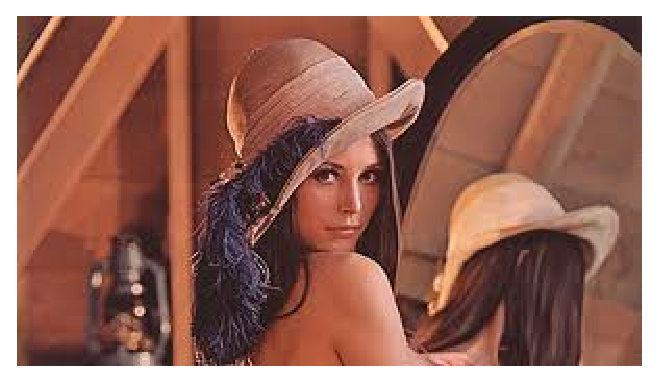
\includegraphics[scale=0.7]{Misc/TODO}
        \caption{Left panel shows the angle dependance of the raw torque signal  clearly showing a positive $B^2$ component for $\theta>0$ and a $-B^2$ component for $\theta<0$. Centre panel shows the \ac{FFT} vs. angle for data with the 2nd order polynomial fitted to $1/B$ removed. A strong angle dependant peak at low frequency is seen. Right panel shows the same data but with a second order polynomial fitted to $B$ removed.}
        \label{Fig:Exp:BackgroundSubtraction}
    \end{center}
\end{figure}

\subsection{Measuring the spin mass}

\TODO{Need to do investigation first}

\subsection{Extracting effective mass from the temperature dependence}
\label{Sec:Exp:ExtractingEffMassTemperatureDependence}

\subsubsection{Basic \ac{LK} formula fitting}

Of all the damping terms in the \ac{LK} equation, only $A_T$ has any kind of temperature dependancy. This term also features the effective mass. By measuring oscillations at a fixed angle but with varying temperatures, the effective mass can be determined. However there is a difficulty in that in-order to observe oscillations, it is necessary to sweep the magnetic field, and many other damping terms have a field dependancy. To the first approximation, an inversely averaged applied field can be used in the \ac{LK} equation provided that the field sweep range is small. However there are a couple of techniques that were employed in order to overcome this shortcoming.

\subsubsection{Retrofitting ansatz \ac{LK} formulae}
\label{Sec:Exp:LKRetrofitting}

One of the primary field-dependant contributions to the oscillation amplitude is the Dingle term scattering (equation \ref{Eqn:Theo:DingleTerm}). This has an exponential dependance with temperature. The Dingle factor, $\alpha = -\pi p m_0/e\tau$, can be determined by fitting a simplified version of equation \ac{LK} equation to oscillations which have been band pass filtered to reduce the number of contributions from other extremal orbits and hence the numeber of necessary fitting parameters. Once we have the Dingle term, a series of ansatz data 



\subsubsection{`Microfitting' the \ac{LK} formula}
\label{Sec:Exp:LKMicrofitting}

\subsection{Method}

Two separate arcs of extremal area were mapped for the angle dependent measurements. One goes along the arc from $B\parallel c$ towards the $a$ axis, the other goes along the arc from $B\parallel c$ towards the $110$ direction. The former we call the $100$ arc, the latter the $110$ arc. In fact, measurements start further back beyond the $B\parallel c$ direction in order to ensure that the minima was reached and to correctly align the crystal as described below.

\subsubsection{Angle correction}
    \label{Sec:Exp:AngleCorrection}

To perform angle dependent measurements, we need to first of all measure accurately the angle between subsequent measurements and second we need to determine the angle of the field compared to the basel planes of the crystal. A further problem is that of aligning the basel plane with respect to the arc of rotation, something that is discussed, briefly here, but in more detail in the results in section~\ref{Sec:ResD:DFTShifts}.

In order to tackle the first problem, the sample platform is subject to a weak oscillating magnetic field from a large coil mounted inside of the yellow cryostat.\footnote{An upper bound on the strength is $\sim$\unit[500]{Gauss}, based on \unit[2.2]{mV} after $\times100$ amplification measured across a coil of $\sim140$ turns with an average area of \unit[3.36]{$mm^2$} per loop} A voltage is induced in a smaller coil which is mounted on the rotating portion of the sample platform\footnote{In fact there are two small coils, each perpendicular to one another although only one is measured at a time} which is proportional to the sine of the angle between the coil and the AC field. By monitoring this voltage, accurate determination of the angle between the sample platform and the field can be made and therefore the angle between subsequent measurements.

The correct angle between the large DC field and the crystal planes in the sample were determined using a post-measurement correction. Since the frequency of the quantum oscillations are field dependent with turning points at the $B\parallel [001]$ direction for approximately two dimensional samples, an even termed polynomial up to fourth order was fitted to the peaks. From the minima of the fits an angular offset was obtained which gave the final correction to the above coil measurements.

The basel angle was aligned on the cantilever by eye. This was coupled with XRD measurements which determined how the visual features corresponded to the crystal axes. This leads to an estimated error in basel plane alignment of around \unit[5]{\%} although we found evidence for greater misalignment in one case, detailed in the results.

\subsubsection{Temperature correction}
    \label{Sec:Exp:TemepratureCorrection}

Effective mass measurements on particular extremal orbits rely on accurate temperature determination at all stages of the field sweep. On the Yellow magnet system, temperature from base of $\approx$\unit[0.3]{K} to $\approx$\unit[2]{K} is controlled by adjusting the He$^3$ sorbtion pump temperature and can be considered to be independant of field effect since the thermometer regulating the sorb temperature is outside of the strong field core. However if we consider figure~\ref{Fig:Exp:TemperatureCorrection}, it is evident that there are magnetic field effects on the RuOx, which is mounted in the base of the magnet but thermally linked with the sample, and the Cernox thermometer that sits on the sample stage.
\begin{figure}[htbp]
    \begin{center}
        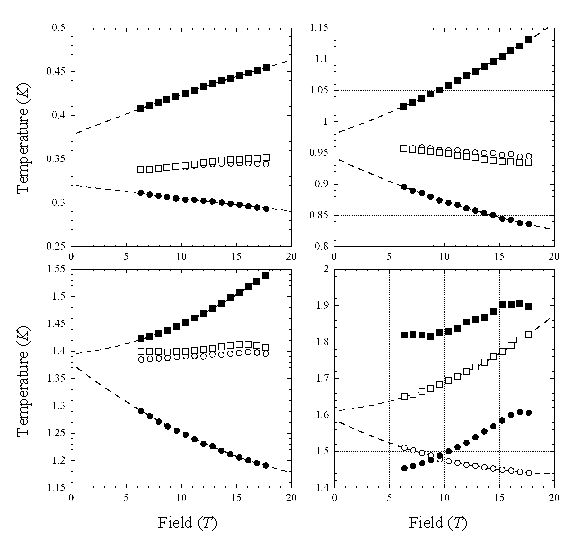
\includegraphics[scale=0.9]{Chapter-dHvABaFe2P2/Figures/Mass/TemperatureCorrection/TemperatureCorrection}
        \caption{Some example temperature readings (squares) set using the sorbtion pump heater. Also shown are corrections (circles) by interpolating to known values. RuOx thermometer is shown in blue, Cernox stage thermometer is shown in red. Second order polynomial fits to the data are shown as lines extrapolated to zero to get a rough estimate of the zero field temperature value.}
        \label{Fig:Exp:TemperatureCorrection}
    \end{center}
\end{figure}
Readings from both thermometers were taken with field sweeps from zero field up to \unit[18]{T} at steady temperatures \unit[0.30]{K}, \unit[0.53]{K}, \unit[0.64]{K}, \unit[1.06]{K} and \unit[1.34]{K}. By interpolating between this data\footnote{Performed using multiquadric radial basis functions from the Scipy Python library.}, the two thermometers can be correctied to agree within $\sim$\unit[0.01]{K}. This interpolation is however limited to temepratures below approximately \unit[1.45]{K} as is shown in the figure for readings at around \unit[1.6]{K}. In these cases, the less reliable method of extrapolating the readings back to zero field using a second order polynomial fit are used as demonstrated with the solid lines in figure~\ref{Fig:Exp:TemperatureCorrection}. In these cases the temeprature is taken to be the mean of the two extrapolated values with the differences defining the error.


\subsection{Yellow Magnet}

dHvA Measurements were all performed in Bristol on the `Yellow Magnet' system which was built by Oxford and can nominally operate up to \unit[20]{t} with use of the lambda plate although more typically is operated up to \unit[18]{T}. The sample sites on a one axis rotator and angle is determined by one of two orthogonal pick-up coils mounted on the sample stage weak, oscillating magnetic, field in

